\chapter{Background} \label{sec:background}

Our work builds on a variety of prior work both by NASA in relation to the Mars
data used, and on existing cross-view pipelines on earth.

\section{The Perseverance (M2020) Rover}

The Mars 2020 mission is the most recent rover mission to Mars, deploying the
Perseverance rover. The Perseverance rover is structurally very similar to the
more well-known Curiosity rover, of the Mars Science Laboratory (MSL) mission. It
was launched for the purposes of broadening the knowledge of the Martian surface
and to explore the Jezero crater region. It also has hardware to collect samples
within the rover and in dead drops for the purposes of eventually being returned
to earth with the Mars Sample Return (MSR/SRL) mission, or with a future
mission.

The Perseverance rover makes a number of changes to the sensor suite included on
the rover. Relevant to this work, both the resolution and bit depth of the
primary navigation cameras on the mast of the rover (Navcam) were upgraded,
having a 1600x1200 pixel resolution ($\sim$2 megapixels) and being in full color
\cite{M2020_Willford2018}. This is in contrast to the Curiosity rover, which
has 1024x1024 pixel resolution with only black and white
\cite{MSLNavcam_Maki2012}. This has the impact that the data processing pipeline
used by this work, as well as the machine learning portion, does not generalize
between the two missions. As such, the newer and higher-quality Perseverance
rover imagery has been chosen for usage in this work.

\section{HiRISE}

The High Resolution Imaging Science Experiment, aka HiRISE mission, is a mission
focused on high resolution imaging of places of interest on the martian surface.
Initially launched in 2005, the orbiter arrived at Mars in 2006, where it has
been operating ever since (long since exceeding its initial (prime) mission
length of 2 years) \cite{HiRISE_McEwen2007}. All orbital imagery used in this
work was acquired from imagery captured by the HiRISE orbiter, later processed
and released as part of the Mars Trek application  \cite{MarsTrek_Law2017}.

\section{VICAR Files}

The Video Image Communication and Retrieval (VICAR) file format is a open
standard internal file format developed by JPL. It's used internally for a
number of missions, starting from Voyager up and until the Perseverance
rover (M2020) mission. It allows for the storage of arbitrary 2d matrix data in
both integer and floating point pixel formats.

Perhaps due to the age of the format, it utilizes slightly different terminology
that is common in image formats today. A VICAR file is organized into one or
more "bands" of data, where each band is has a specified data type. Each band
has a given number of "lines", the height of the image band, and a given number
of "samples" per line, the image width. The start of the file also includes a
labels, text data used both for specifying image metadata (dimensions, pixel
format, etc), and for arbitrary metadata. In the case of M2020 Perseverance
imagery, notable metadata includes the location of the image (relative to the
site frame), and the time the image was taken \cite{VICAR}.

\section{GeoTIFF}

GeoTIFF is an open metadata standard for storing georeferencing information
inside the already widely-utilized TIFF file format. It allows for a TIFF file
to contain coordinate system information and information on the projection used
by a given GeoTIFF file to allow for usage in precise geolocation. GeoTIFF is
also widely supported, with it being a primary file format used by GDAL, an open
source suite of tools for manipulation geographic data.

In this work, the USGS satellite data from HiRISE was in GeoTIFF format, and
manipulated by GDAL \cite{USGS_Mars2020_TRN_HiRISE_2020, GDAL_2025}.

\section{Central Cylindrical Projection} \label{sec:central-cylindrical-background}

The input panoramas use central cylindrical projection, where the azimuth of the
camera directly corresponds with the pixels in the image (with appropriate
scaling), and the elevation corresponds to the tangent of the pixels in the
image. Formally, that is:

\begin{align}
    x &= w \left( \frac{\theta - \theta_{\text{min}}}{\theta_{\text{max}} - \theta_{\text{min}}} \right) \\
    y &= h \left( \frac{\tan \phi - \tan \phi_{\text{min}}}{\tan \phi_{\text{max}} - \tan \phi_{\text{min}}} \right)
\end{align}

where:

\begin{itemize}
	\item $x$ and $y$ are the corresponding pixel positions
	\item $w$ and $h$ are the width and height of the image
	\item $\theta$ is the azimuth of the view (in radians)
	\item $\phi$ is the elevation of the view (in radians)
	\item $\phi_{\text{min}}$ and $\phi_{\text{max}}$ are the minimum and
	maximum elevations of the view, respectively
\end{itemize}

A visual of this is shown in \cref{fig:central-cylindrical}.

\begin{figure}

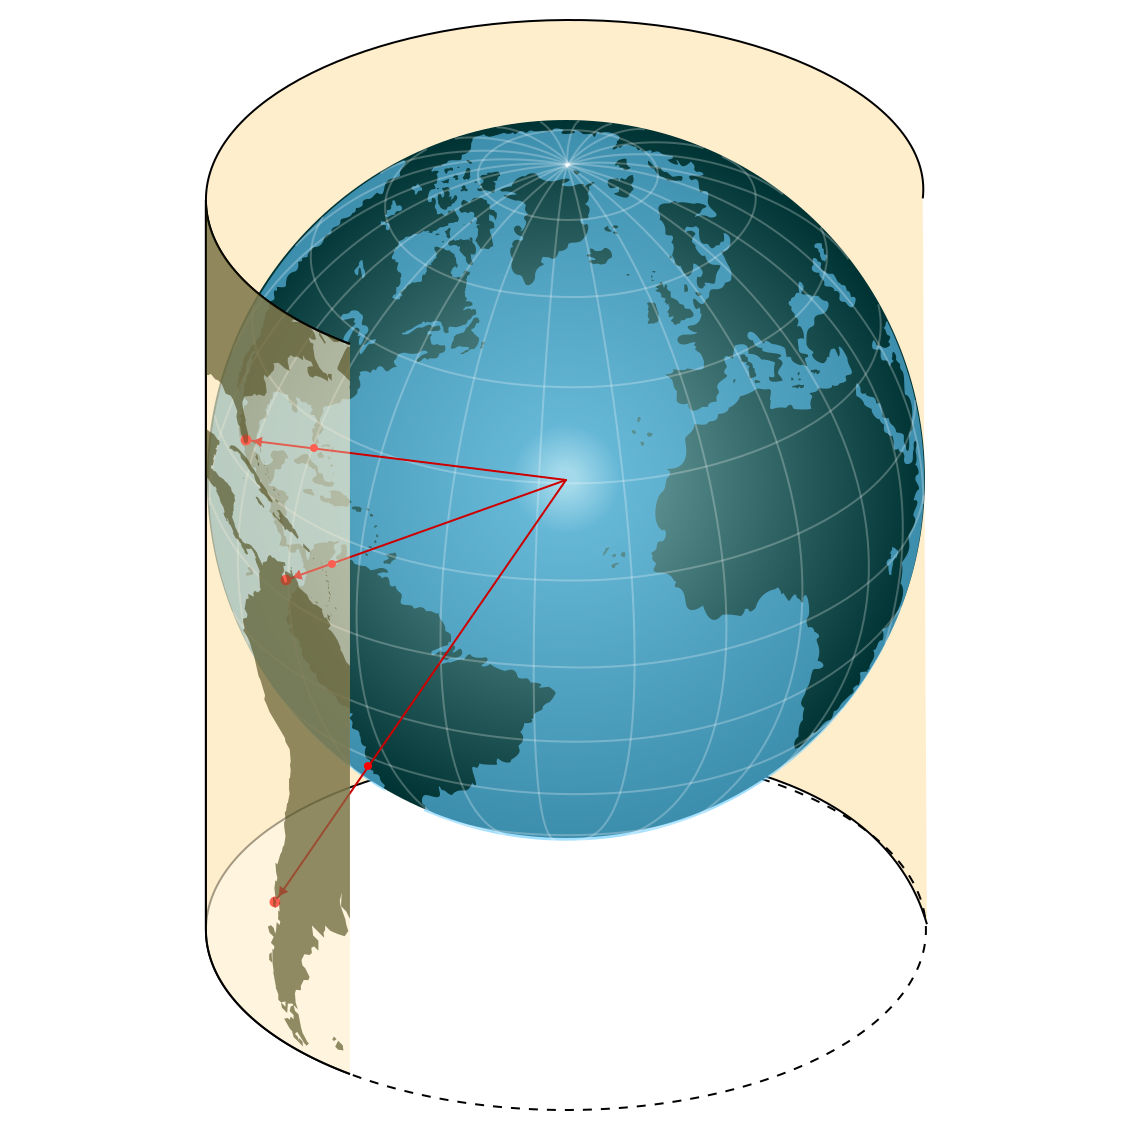
\includegraphics[width=0.4\linewidth]{central-cylinder-proj-example.jpg}

\caption{
    Visualization of central cylindrical projection. Image by C. M. G. Lee
    (2008), Wikimedia Commons, Licensed under CC BY-SA 4.0
    \cite{Lee2008CentralCylindricalLightProjection}.
}
\label{fig:central-cylindrical}

\end{figure}
